\section{Project Demonstration}
This section will explain how to use the engine, including screenshots demonstrating each portion of it being used. \\
To use the search engine, the user types a query into the search bar and then presses enter or the search button (fig1). This will lead to the loading page (fig2) and then the results page (fig3). This shows a sorted list of pages in relation to their similiarity to the query. At the top of the page is our logo, which can be clicked to return to the homepage.\\
There is also the functionality of adding pages. For this, the user clicks on the addpage button below the search bar on the homepage. This leads you to the addPage page (fig4). Here, the user can add one or more links and then press the add button. The page will then load for a couple of minutes (fig5) and present a "page loaded successfully!" message (fig6). 

\includegraphics[width=\textwidth,keepaspectratio]{query.png}\\
Figure 1: The homescreen


\includegraphics[width=\textwidth,keepaspectratio]{resultsLoading.png}\\
Figure 2: The query loading screen

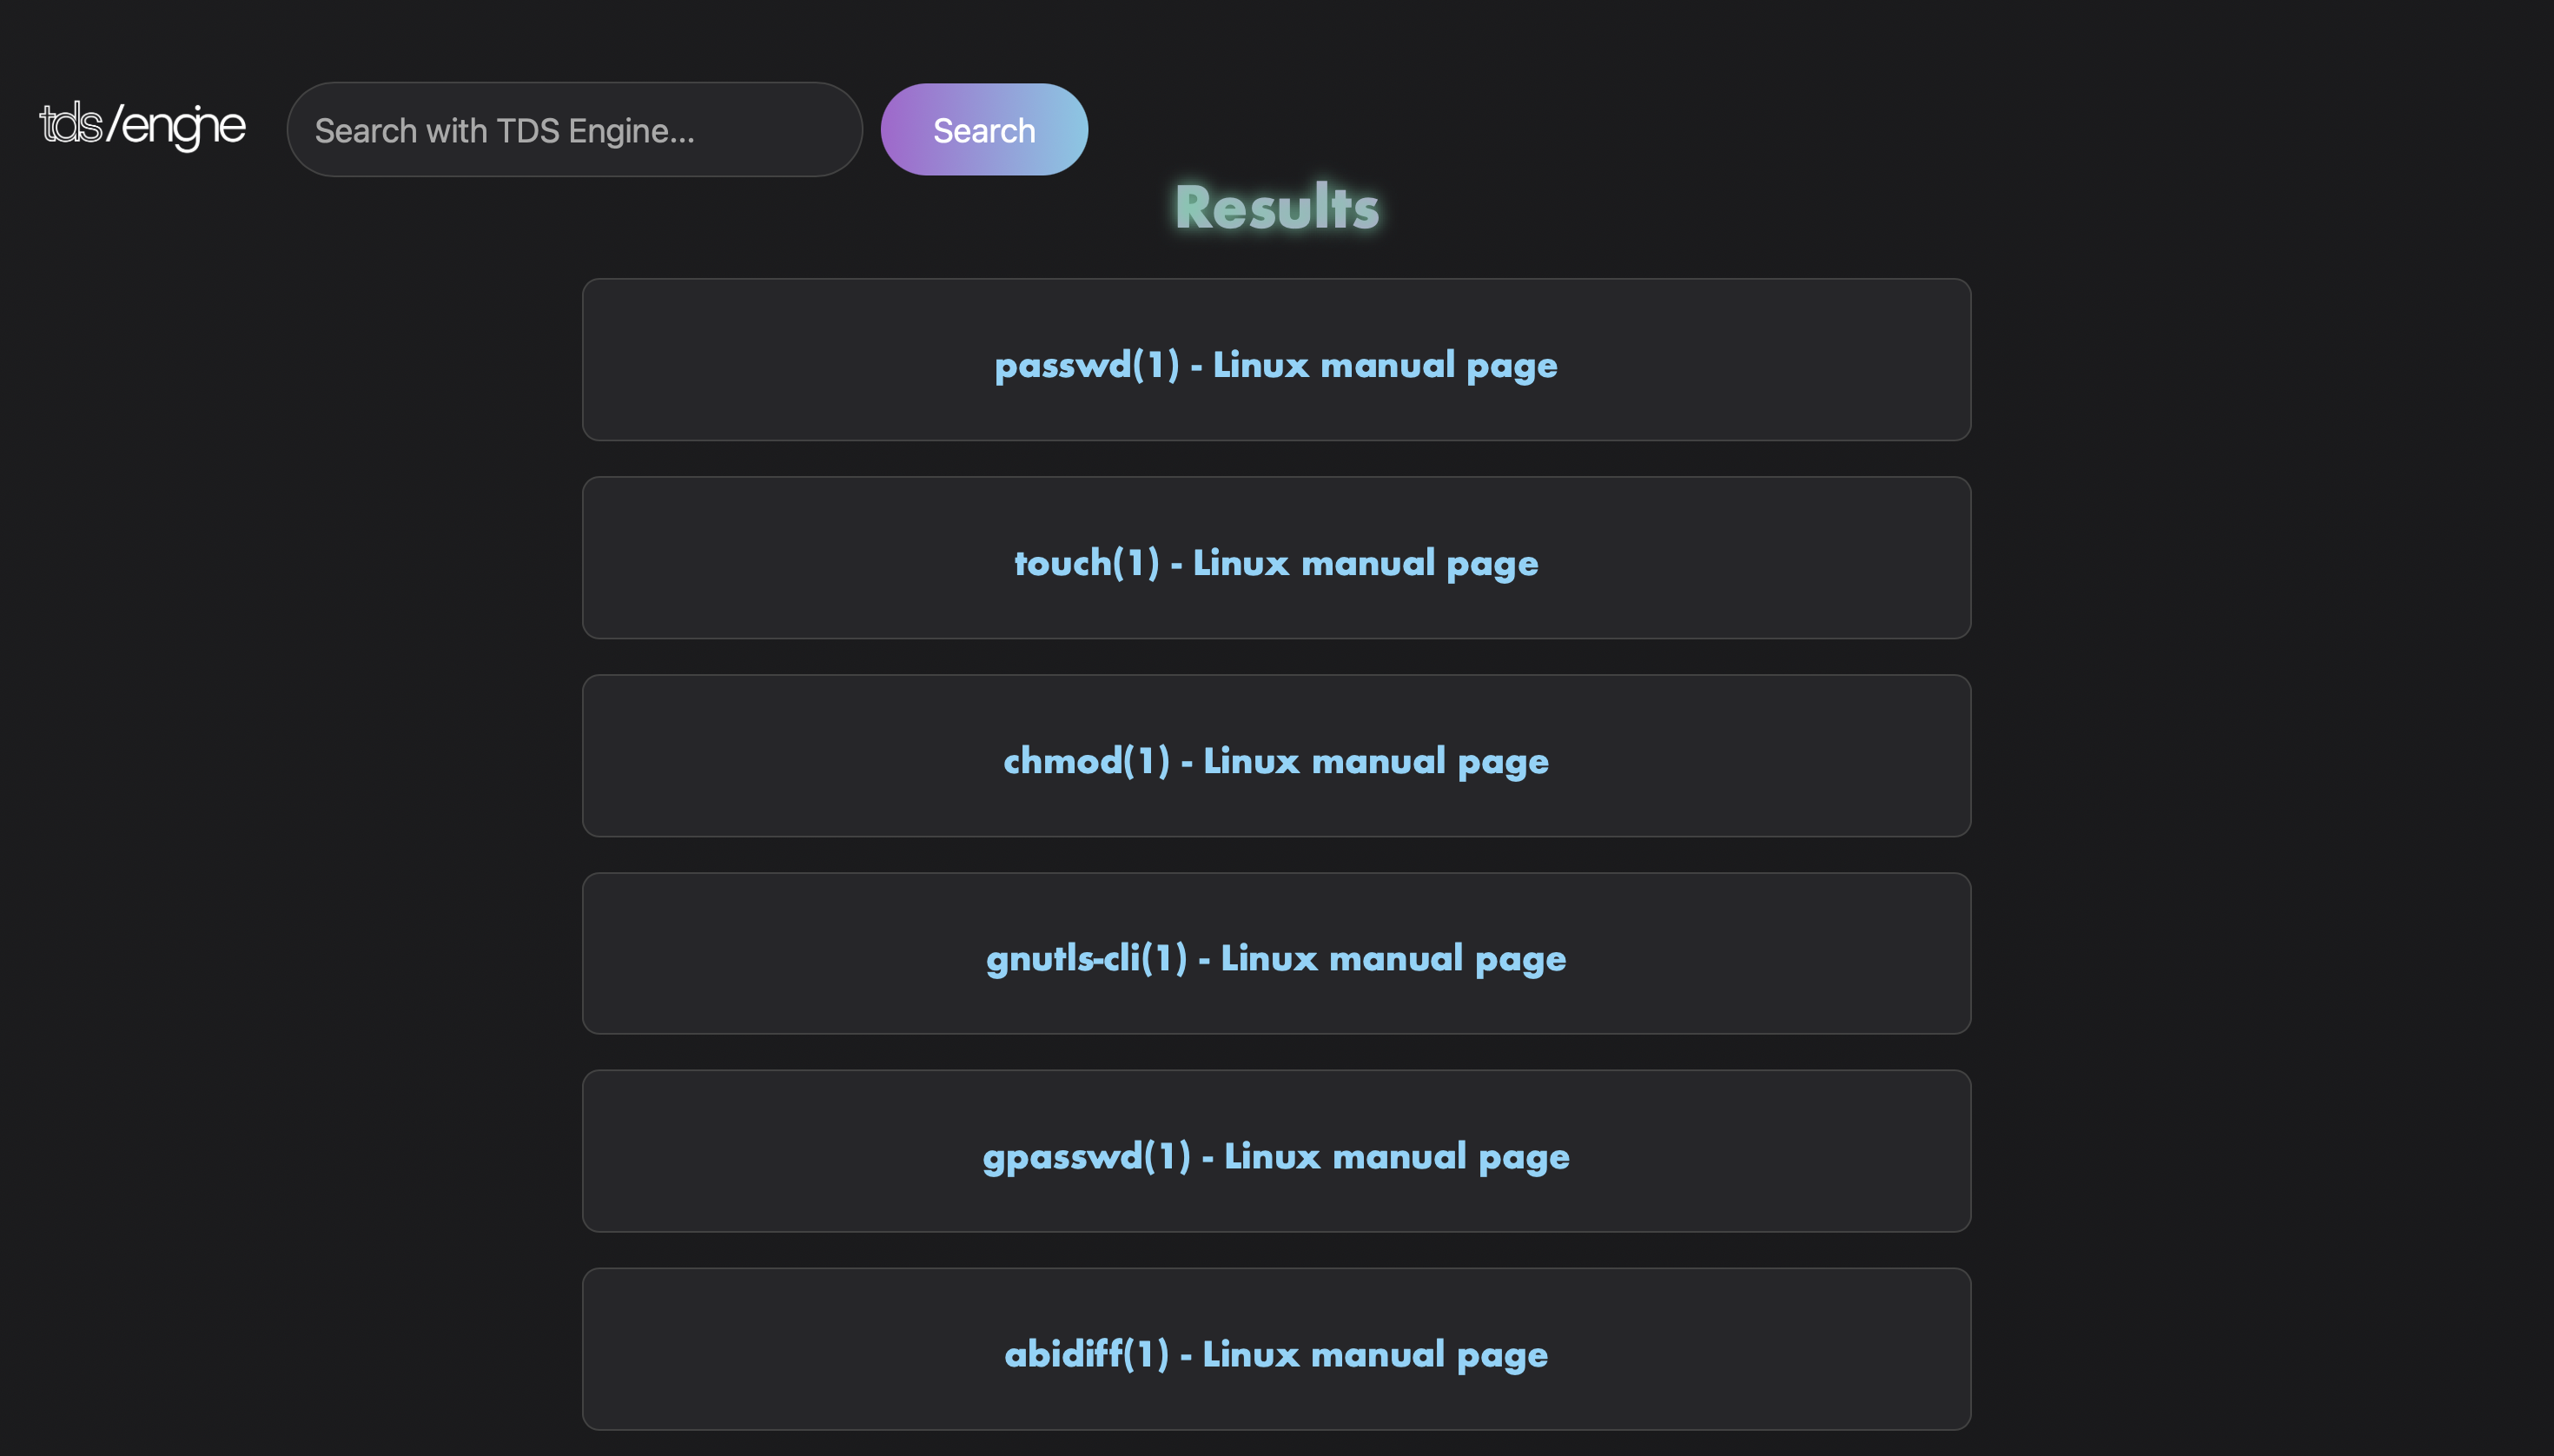
\includegraphics[width=\textwidth,keepaspectratio]{results.png}\\
Figure 3: The results

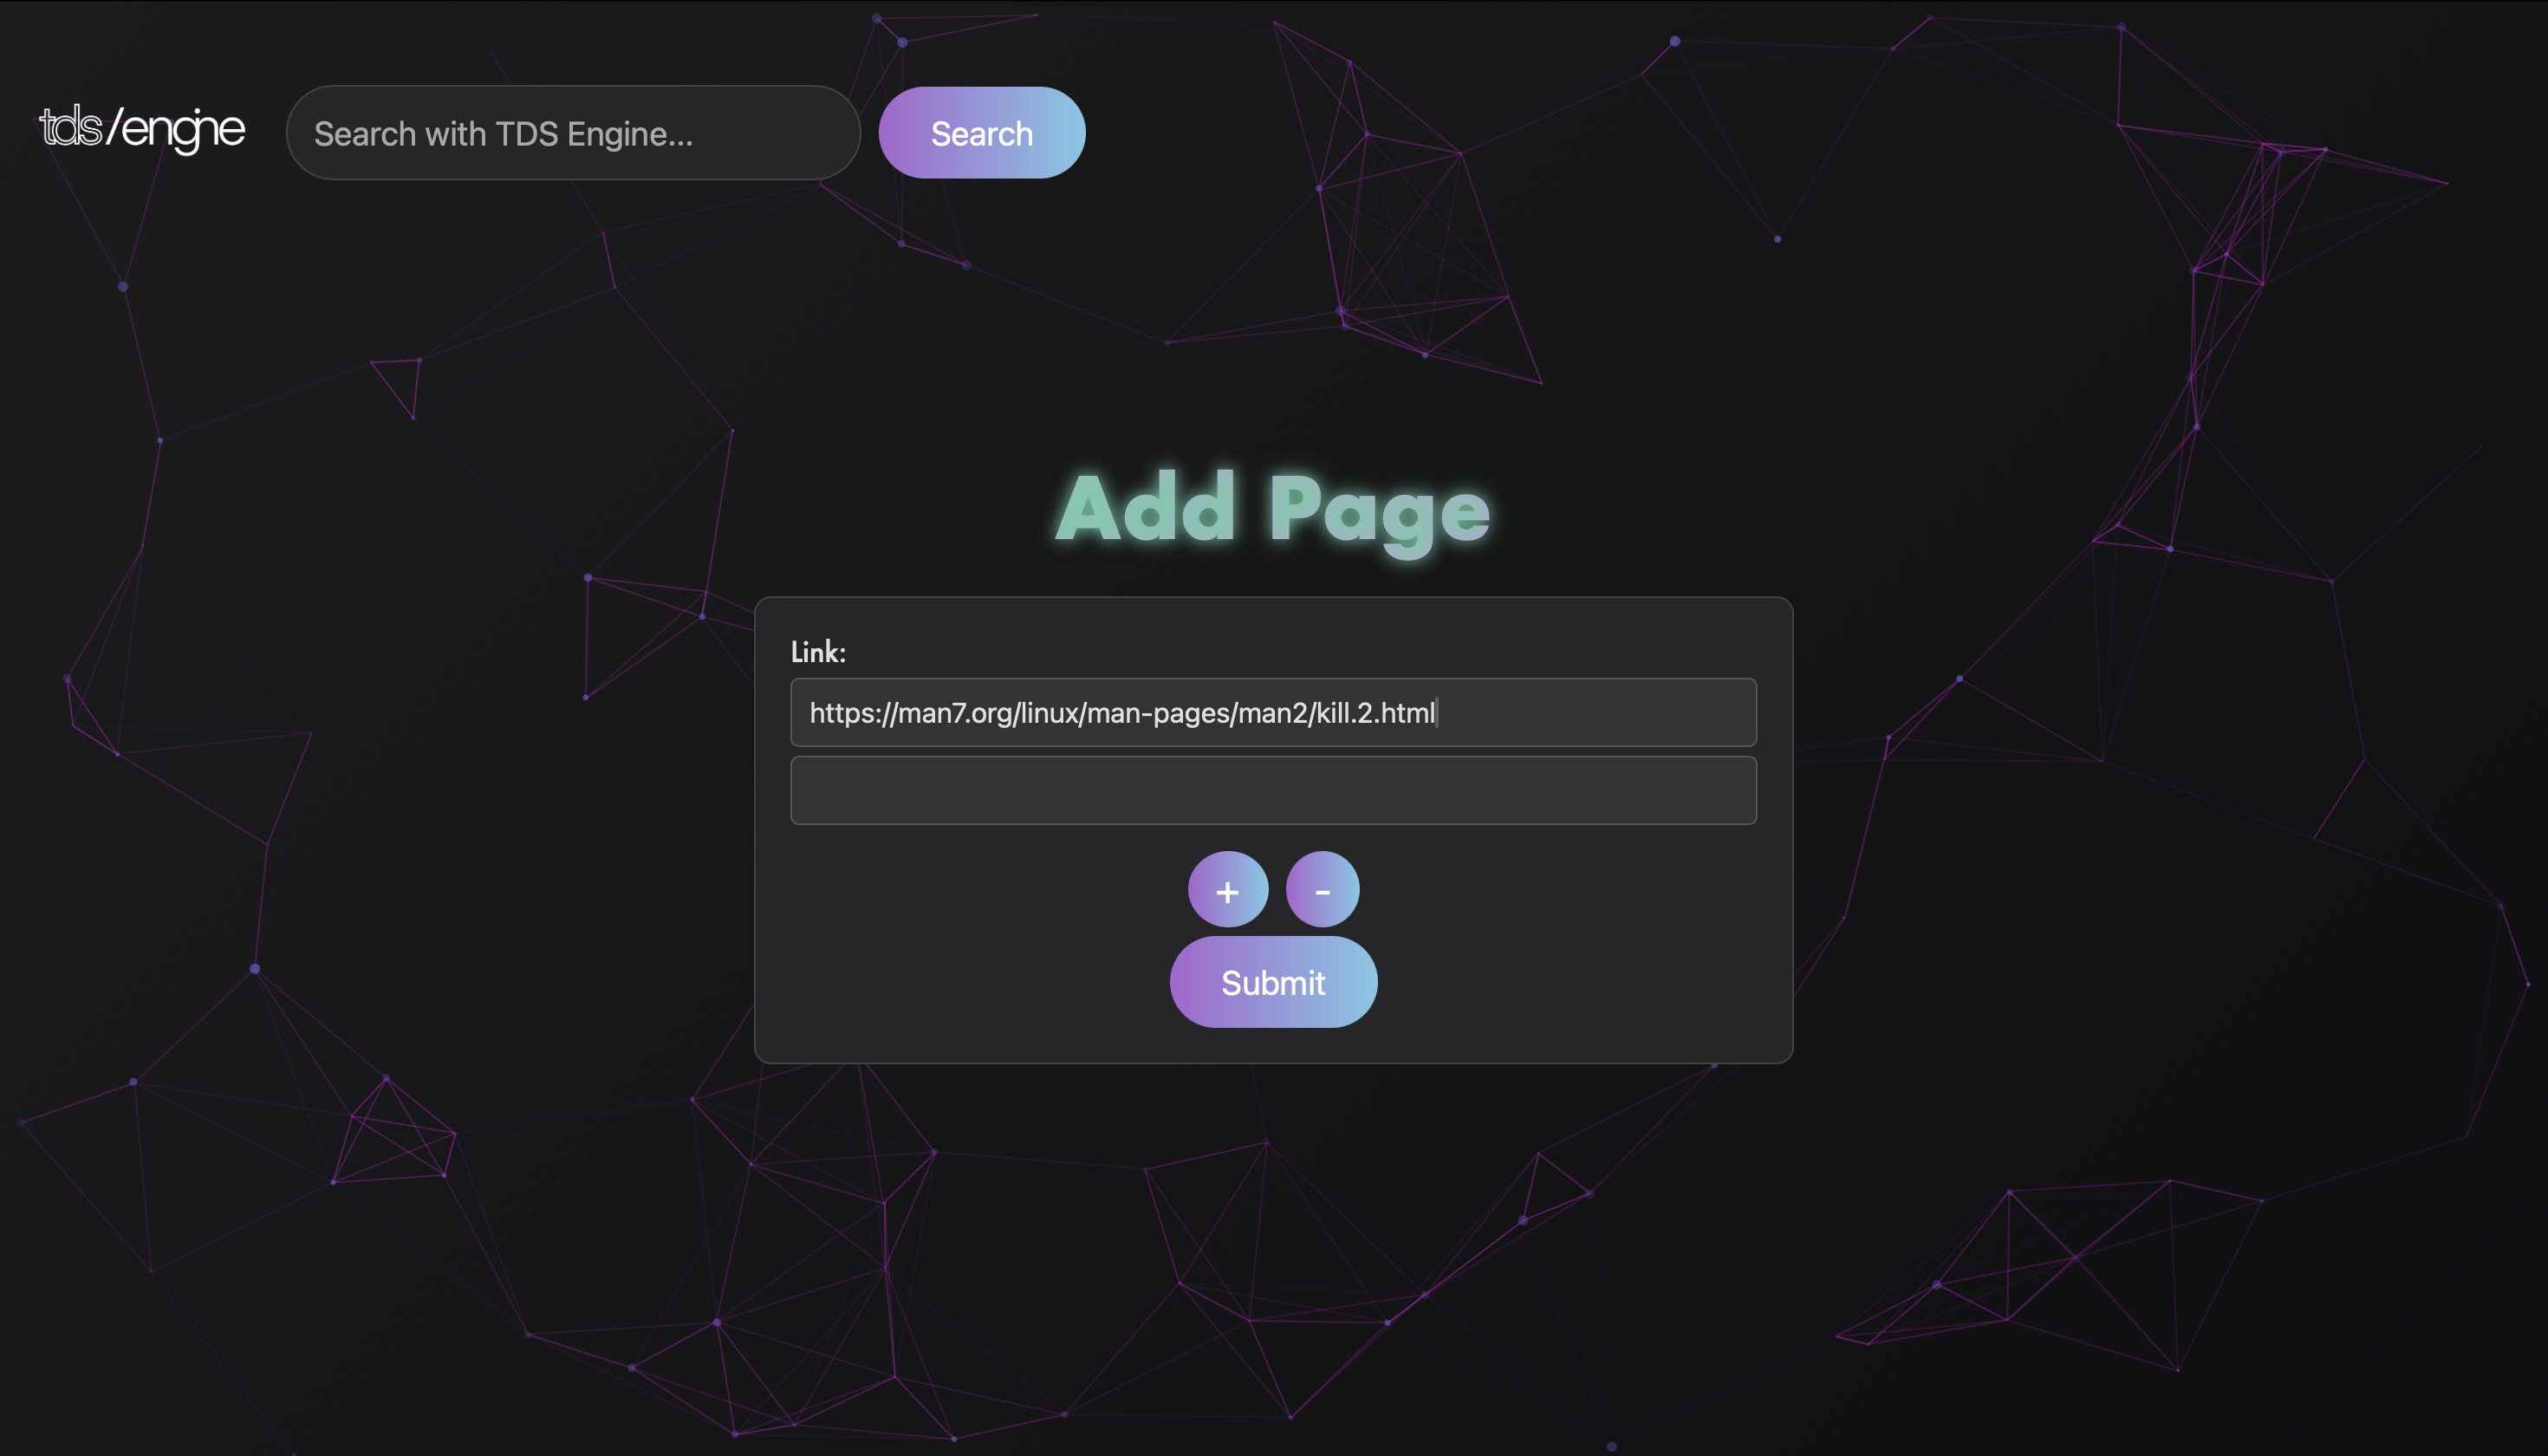
\includegraphics[width=\textwidth,keepaspectratio]{addPage.png}\\
Figure 4: The page adding page

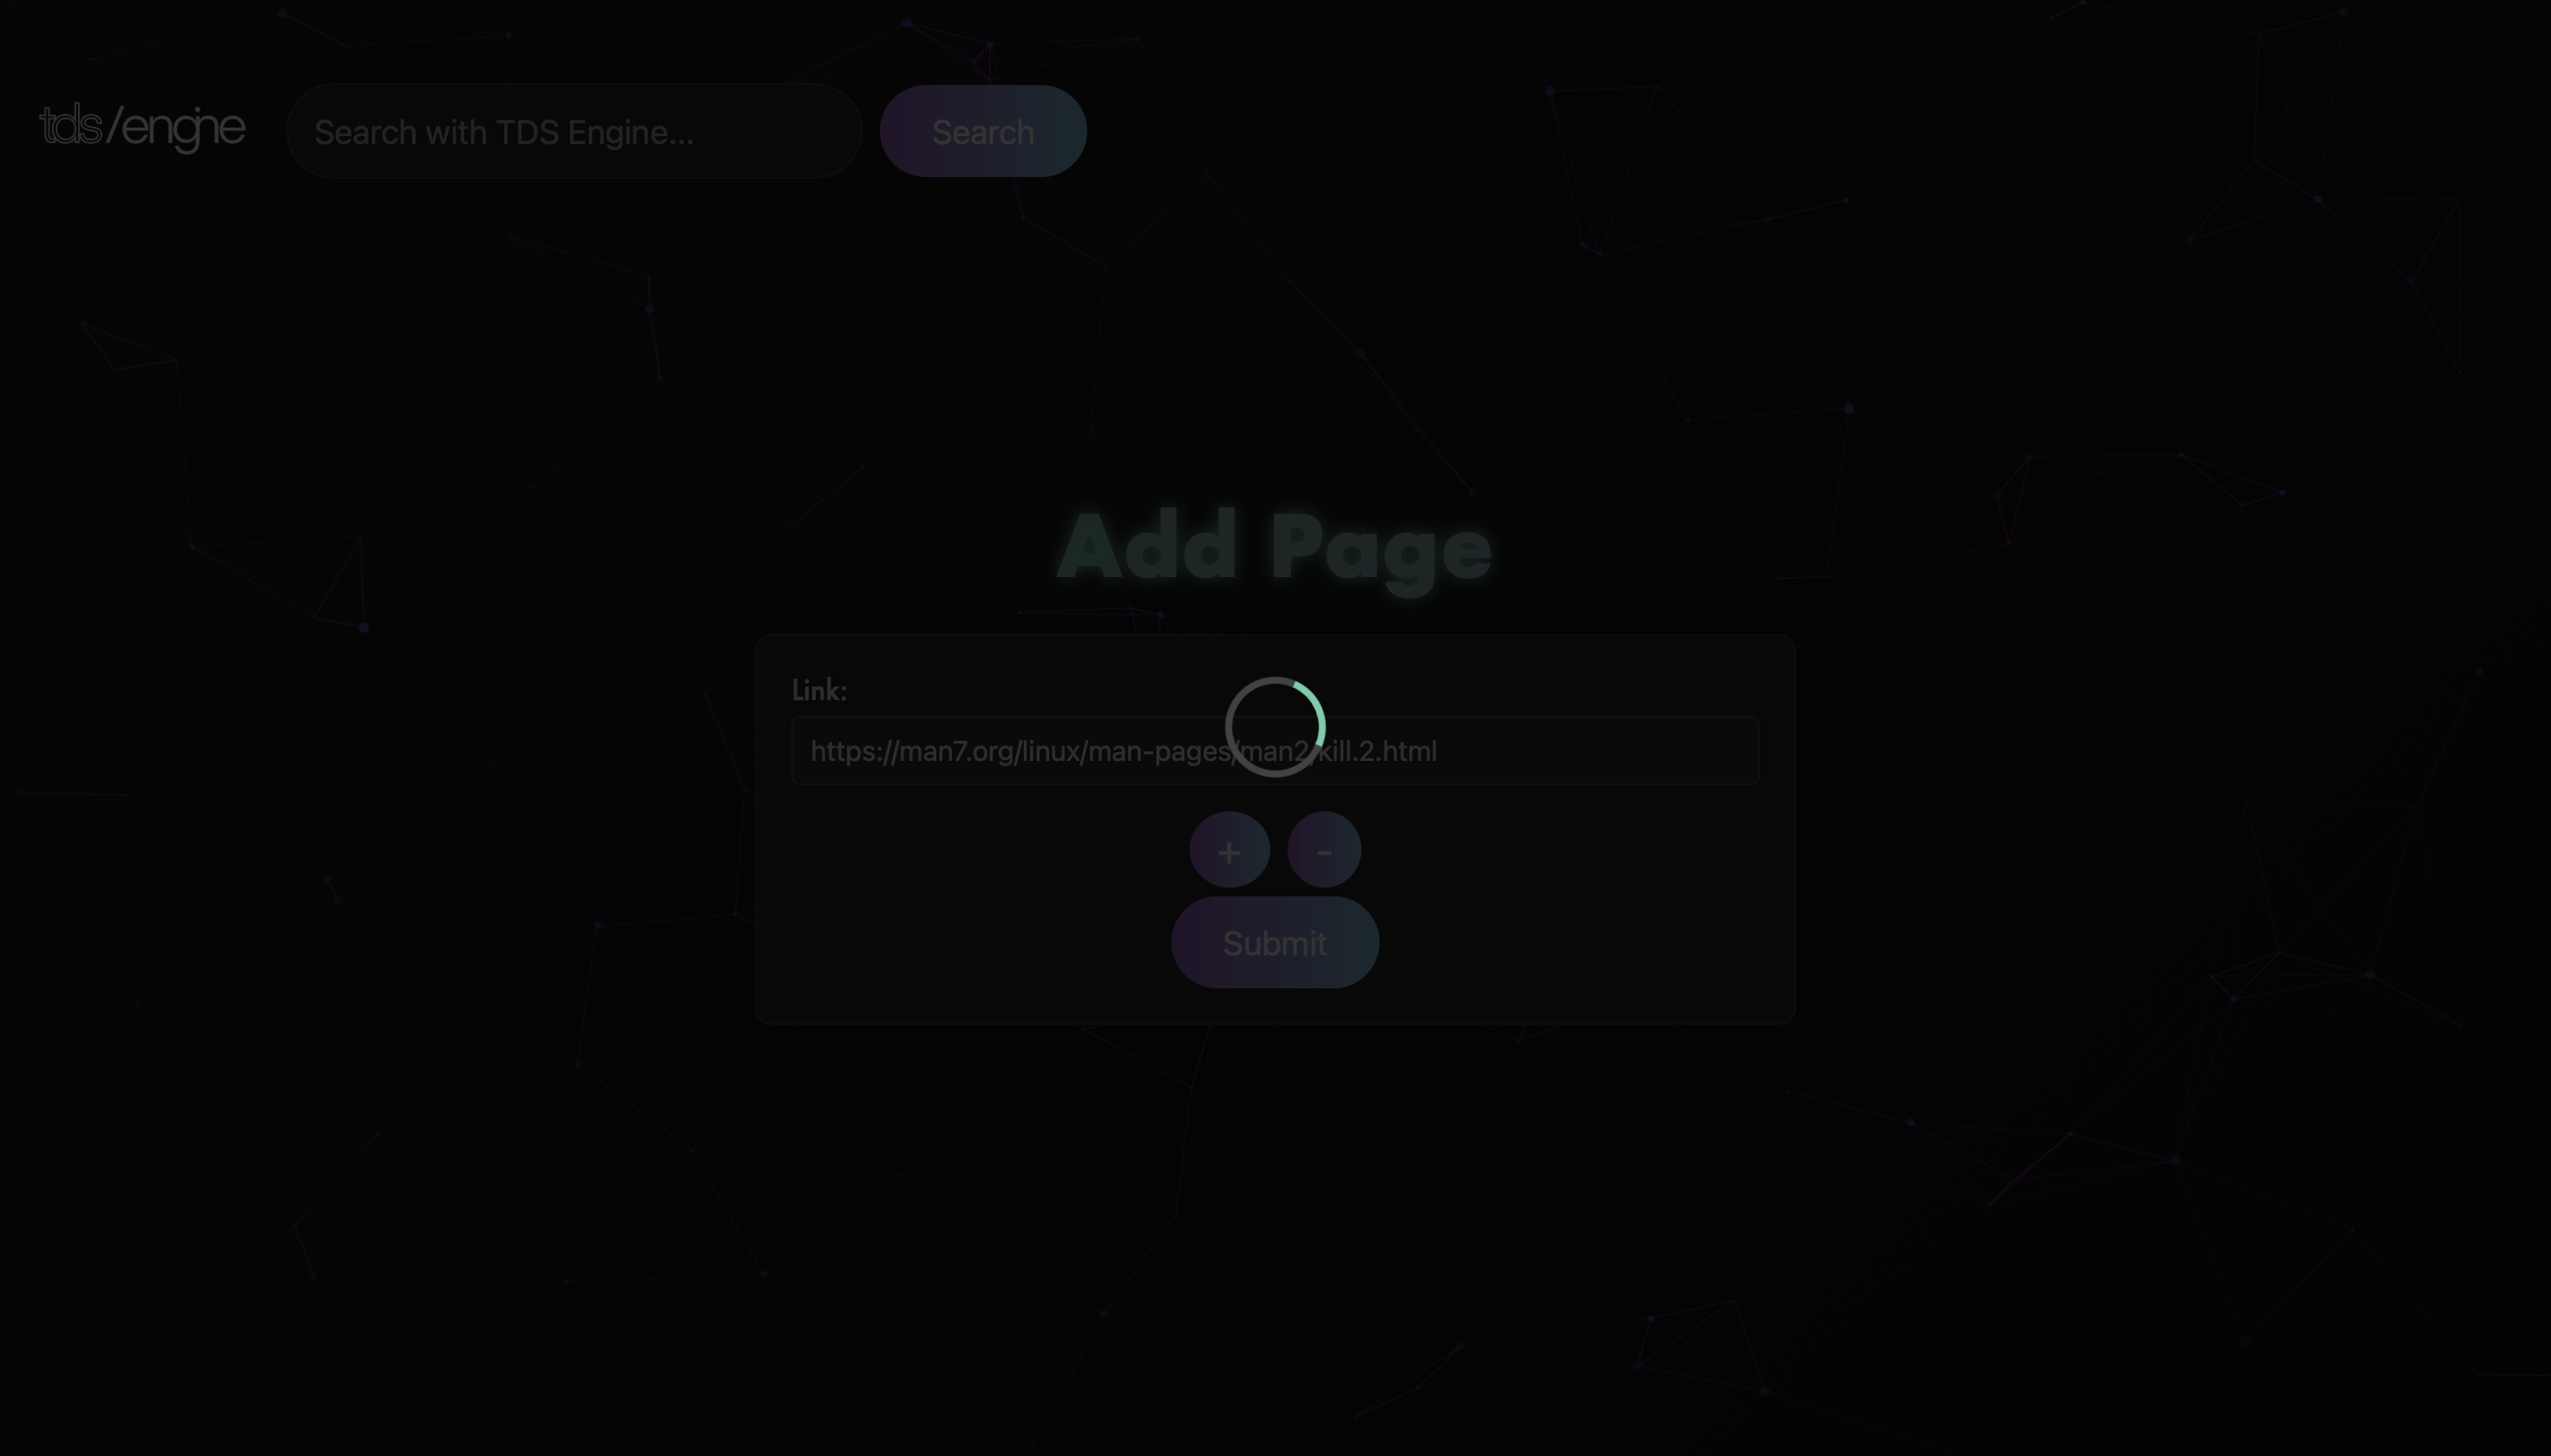
\includegraphics[width=\textwidth,keepaspectratio]{addPageLoading.png}\\
Figure 5: Page adding loading

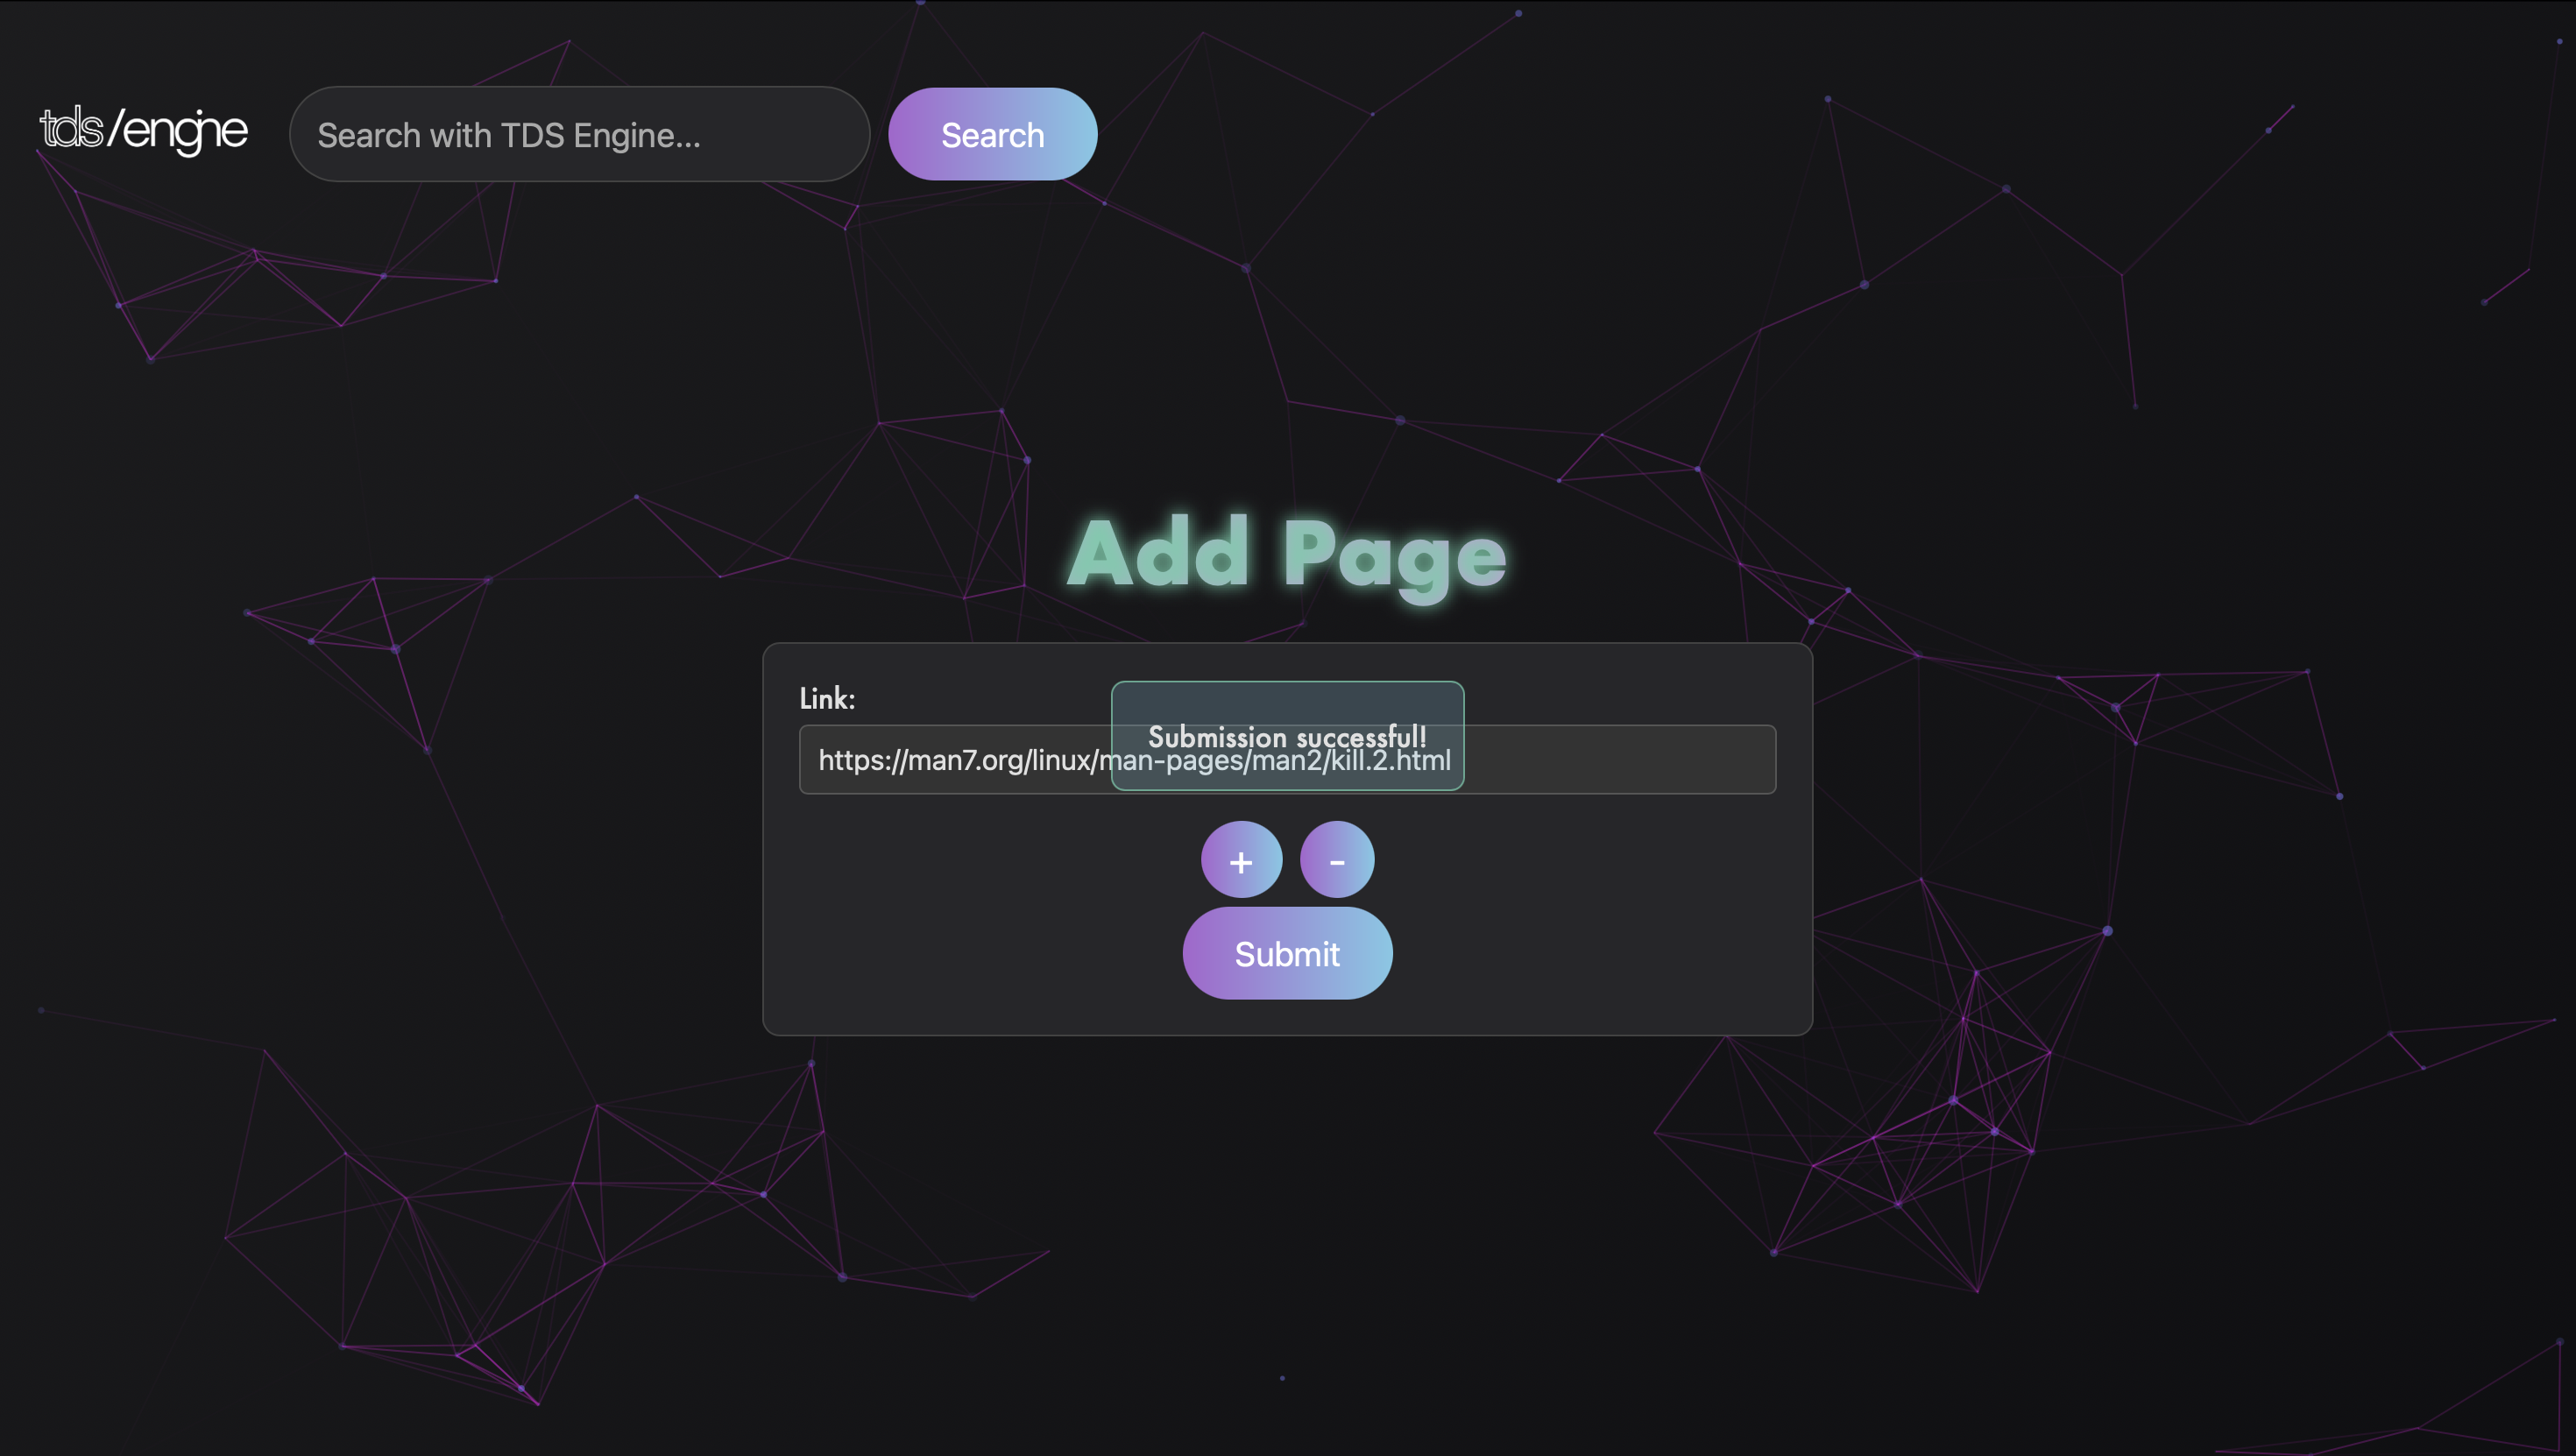
\includegraphics[width=\textwidth,keepaspectratio]{addPageSuccess.png}\\
Figure 6: Page added confirmation
